\chapter{Entwurf}

\section{Softwarearchitektur}\label{chp:softwarearchitektur}
Um den verschiedenen Anforderungen gerecht zu werden,
folgt die Softwarearchitektur drei Architekturmustern
\footnote{
In der Softwaretechnik versteht man unter einem \first{Muster} generell eine
Lösungsstrategie für ein bestimmtes Problem.
\index{Muster}
Ein Muster folgt dabei generell dem Format \enquote{Preconditions} -
\enquote{Problem} - \enquote{Constrains} - \enquote{Solution}.
\citep{beck_patterns_1994}
\first{Architekturmuster} sind Muster auf höchster Abstraktionsebene
einer konkreten Aufgabenstellung.
\index{Muster!architektur}
Die zugrundeliegenden Probleme sind dabei organisatorischer und
architektonischer Art, wo hingegen \first{Entwursmuster}, oder
auch \fisrt{Idiome}, Muster für die Lösung sehr granularer und konkreter
Probleme darstellen.
\index{Muster!enturfs}
\index{Idiom|see{Entwurfsmuster}}
\citep{buschmann_pattern-oriented_1996}
}
aus der
Softwareentwicklung, mit denen sich die Anwendung auf unterschiedlichen
Abstraktionsebenen beschreiben lässt:
\index{Softwarearchitekur}
\index{Architektur|see{Softwarearchitekur}}

\todo{einzelne Muster generell erklären?}

\subsection{Pipes and Filters}
Die höchste Abstraktion stellt das \first{Pipes and
Filters}-Patten dar:
\index{Architekturmuster!Pipes and Filters}

\begin{figure}[htbp]
	\begin{center}
		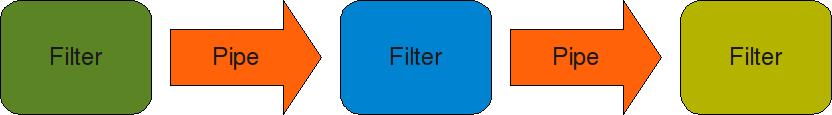
\includegraphics[scale=0.7]{pics/pipesFilter3.png}
	\caption[Pipes and Filter]{
	\textbf{Das Pipes and Filter Pattern}
	ist ein Architekturmuster für Systeme, um einen Strom von Daten zu
	verarbeiten.
	Jeder Verarbeitungsschritt ist in einen eigenen Filterkomponenten gekapselt.
	Die Daten werden dabei durch \name{Pipes} geleitet, die benachbarte
	\name{Filter} verbinden.
	Durch die Kapselung der Filter können diese rekombiniert werden, umso Familien
	von verwandten Systemem zu erstellen.
	\citep{buschmann_pattern-oriented_1996}}
	\end{center}
	\label{fig:pipesFilter}
\end{figure}

Die zu annotierende Sequenz wird schrittweise durch verschiedene \first{Filter}
bearbeitet. Jeder Filter, der in der \first{Pipeline} vorhanden ist, wird dabei
das entgültige Ergebnis der Annotation durch seine spezifischen Ergebnisse
erweitern.

Der Input eines Filters besteht dabei zum einen aus der zu
annotierenden Sequenz selbst, zum anderen aus einem zentralen Datenobjekt, in
dem alle gewonnenen Ergebnisse abgespeichert werden.
Ein Filter kann dabei auch auf die Ergebnisse eines anderen
Filters zugreifen oder auch angewiesen sein.
Die Reihenfolge der Filter innerhalb der Pipeline wird
somit durch die spezifischen \first{execution preconditions}
\footnote{\todo{execution precondition}}
aller Filter festgelegt.
\index{Filter}
\index{execution precondition}

Es ist davon auszugehen, dass die Ausführung einzelner Filter mitunter sehr
zeitintensiv sein wird. Ausserdem soll Nutzen aus dem im Institut installierten
\first{LSF} gezogen werden. Daher wird eine rein sequenzielle Abfolge der
Filter, wie es das Entwursmuster suggeriert, vermieden werden.
Stattdessen kann die Ausführung einzelner Filter parallel erfolgen.
Sind zu einem Zeitpunkt die execution preconditions mehrerer Filter erfüllt,
werden diese sofort zur Ausführung gebracht.
\index{Platform LSF}

Die Pipeline soll möglichst leicht konfigurierbar sein und sich an
individuelle Bedürfnisse anpassen lassen.
Vor diesem Hintergrund soll die Pipeline die veränderbaren Steps und das
statische \enquote{Ausführungsgerüst} vollständig entkoppeln. Beim Starten der
Pipeline soll diese an einem bestimmten Ort (lokales Verzeichnis oder
entferntes Repository) nach vorhandenen Steps suchen und diese in der Pipeline
installieren.

Die \name{Filter} des \name{pipes and filters} pattern sind somit aus der
eigentlichen Anwendung herrausgelöst. Sie sind über eine generische
Schnittstelle repräsentiert, deren Implementierung zur Kompilierzeit nicht
bekannt ist.

\begin{figure}[htbp]
	\begin{center}
		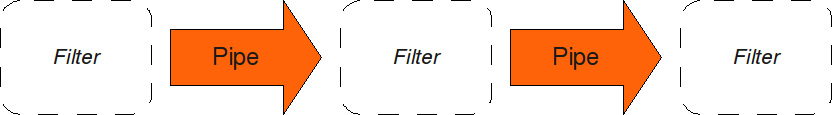
\includegraphics[scale=0.7]{pics/pipesFilter21.png}
	\caption[Pipes and Filter 2]{
	\textbf{Das Pipes and Filters Pattern.}
	Ein statisches Gerüst, dazu dynamische Filter, die in Form von Plugins geladen
	werden \todo{ein bisschen genauer, schöner, detailreicher?}}
	\end{center}
	\label{fig:pipesFilter21}
\end{figure}

Die Pipeline teilt sich so in zwei Teilkomponenten:
Die \enquote{dynamischen Steps} und das \enquote{statisches Ausfürhungsgerüst}.
\subsection{Client-Server}
Durch ihre dynamische Struktur kann die Pipeline auf einer weiteren
Abstraktionsschicht durch das \first{Client-Server}-Pattern dargestellt werden:
Ein statischer Server kommuniziert über eine definierte Schnittstelle mit
dynamischen Clients.
Clients können kommen und gehen und sind nicht auf eine konkrete
Implementierung festgelegt. 

Die \first{Pipes} des \name{pipes and filters} Pattern werden somit zu einem
zentralen \first{Server} zusammengefasst und bilden das statische
Ausführungsgerüst.
\first{Clients} werden durch die \first{Steps} repräsentiert. \seec{chp:pipes
and filters} Es können beliebig viele Clients am Server anmeldet werden, wodurch
die eigentliche Pipeline aufgebaut wird.

\begin{figure}[htbp]
	\begin{center}
		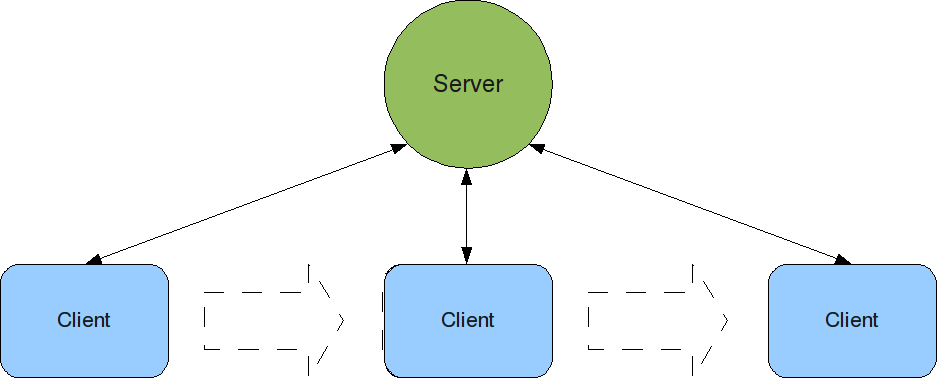
\includegraphics[scale=0.6]{pics/serverClient2.png}
	\caption[Client Server]{
	\textbf{Abstraktion durch das Client-Server-Pattern.}
	Einzelne \name{Steps} können sich
	dynamisch an einem \name{Server} an- und abmelden. Der Server organisiert die
	angemeldeten Clients nach deren Anmeldung zu der eigentlichen Pipeline.}
	\end{center}
	\label{fig:clientServer2}
\end{figure}

\paragraph{Server}
Die Anforderungen an den Server gliedern sich in zwei Teilbereiche:
\begin{description}
\item[Organisation und Synchronisation der Client Ausführung]
Die Ausfürhrung der angemeldeten Steps kann sequenziell oder
parallel erfolgen, je nachdem, welche \name{preconditions} für den jeweiligen
Step erforderlich sind und ob die zur Ausführung benötigten Daten eventuell
erst durch einen anderen Step bereitgestellt werden müssen.
Vor der eigentlichen Ausführung wird der Server somit zum einen die
\name{preconditions} prüfen, zum anderen, ob der Step überhaupt zur Ausführung
gebracht werden muss, oder ob die zu erwartenden Ergebnisse bereits in selber
oder in anderer Form vorhanden sind.
\item[Datenverwaltung] Die Ergebnisse der einzelnen Steps werden zentral durch
den Server verwaltet.
Zum einen synchronisiert der Server die Zugriffe auf die Daten, zum anderen
werden diese persistiert, um bei einer gewollten oder ungewollten Unterbrechung
der Pipeline Datenverlust zu verhindern.
\end{description}

\paragraph{Client}
Auf der Clientseite stehen die einzelnen Steps, die eine gemeinsame
Schnittstelle zur Kommunikation mit dem Server implementieren über welche der
Server \name{preconditions} überprüfen, \name{solutions}
\seec{chp:softwarearchitektur} entgegennehmen und die eigentliche Ausführung
anstossen kann.

%%
%\begin{figure}[htbp]
%	\begin{center}
%		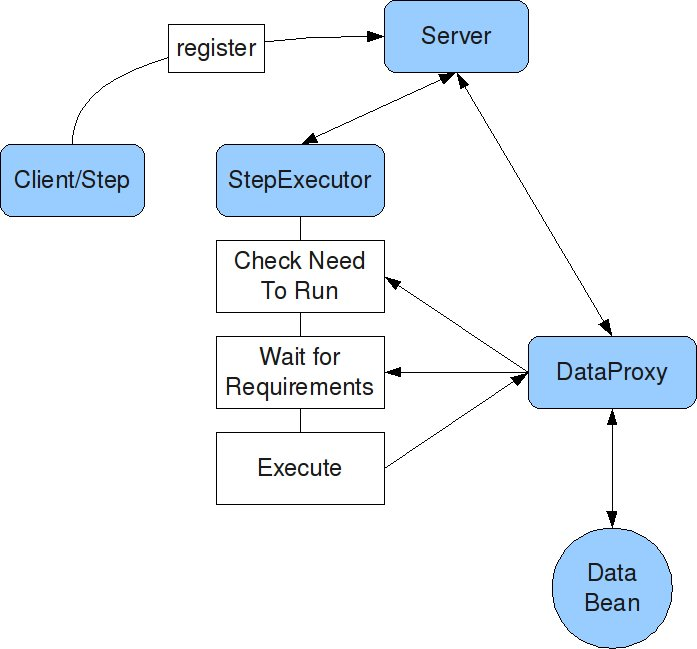
\includegraphics[scale=0.6]{pics/programOrganisationOverview3ScaledWithAlpha.jpg}
%	\caption[Design 1]{
%	\textbf{Design 1.}
%	something. \todo{Teilung von Server hier noch nicht erwähnt. Evtl. Teil der
%	Umstzung}}
%	\end{center}
%	\label{fig:programOrganisationOverview3ScaledWithAlpha}
%\end{figure}

\subsection{Serviceorientierte Architektur}
Die unterste Abstraktionebene wird durch eine \first{serviceorientierte
Architekur} gebildet.
Diese Architektur wird massgeblich durch das \first{OSGi Framework}
diktiert, was die Basis der Anwendung bilden soll.

\subsubsection{Das OSGi Framework}\label{chp:osgi}

Die \name{OSGi Alliance}, früher \enquote{\textit{Open Services Gateway
initiative}}, ist ein Zusammenschluß verschiedener Unternehmen, wie z.B. IBM,
Oracle oder Sun Microsystems.
Sie spezifiziert die \first{OSGi Service Platform}, eine Java-basierte
Softwareplattform, die nach einem \first{Komponentenmodell}
% footnote is von wikipedia !!!
\footnote{nach Gruhn und Thiel\citep{gruhn_komponentenmodelle_2000}:
\enquote{Ein Komponentenmodell legt einen Rahmen für die Entwicklung [..] von
Komponenten fest, der strukturelle Anforderungen hinsichtlich Verknüpfungs-
bzw. Kompositionsmöglichkeiten sowie verhaltensorientierte Anforderungen
hinsichtlich Kollaborationsmöglichkeiten an die Komponenten stellt.}}
organisiert ist.
\citep{wtherich_die_2008}
Einzelne Komponenten, sogenannte \first{Bundles}, können der Anwendung
dynamisch hinzugefügt und wieder entfernt werden ohne dass ein erneutes
Kompilieren oder Starten der Anwendung nötig ist.
Abhängigkeiten zwischen Bundles werden dabei automatisch aufgelöst; ein
intelligentes Versionsmanagement steht ebenfalls zur Verfügung.

Die \name{OSGi Service Platform} weisst ausserdem eine serviceorientierte
Architektur \footnote{Unter \first{serviceorientierte Architektur} oder auch
\first{dienstorientierte Architektur} versteht man ein Softwaredesign, dass
sich durch sogenannte Dienste oder auch Services auszeichnet. Diese können
appliktaions-global an einer Registry angemeldet und abgefragt werden. Sie
stellen dabei eine Schnittstelle zu bestimmten Funktionen bereit, ohne dabei
die zu Grunde liegende Implementierung preiszugeben.}
auf: 
Sie stellt eine globale Registry (\first{Service Registry})
bereit, an der Bundles \first{Dienste} bzw. \first{Services} anmelden und
abfragen können.

\subsection{Bundles}
Ein Bundle ist nach OSGi Spezifikation\citep{osgi_2009} eine technische Einheit
von Klassen und Ressourcen, die eigentständig in der Anwenung gestartet,
gestoppt, installiert und deinstalliert werden kann.
\index{Bundle}

Ressourcen und Klassen eines Bundles können anderen Bundles bereitgestellt
werden. Dazu müssen sie vom bereitstellenden Bundle explizit exportiert werden
und durch das nutzende Bundle explizit importiert werden. Jedes Bundle stellt einen
Bundlenamen, der üblicherweise von der enthaltenen Paketstruktur
abgeleitet wird, sowie eine Versionsnummer bereit. Aus diesen beiden Komponenten
wird dann eine eindeutige Identifizierung des Bundles generiert.
So ist es beispielsweise möglich, ein und das selbe Bundle in unterschiedlichen
Versionierungen zu installieren.

Über die \first{MANIFEST.MF}, die ohnehin in jedem Jar-File vorhanden ist, wird
das Bundle neben dem Namen und der Version mit weiteren Meta-Informationen, wie
importierte und exportierte Pakete oder Lauzeitumgebung, ausgestattet.
\index{MANIFEST.MF}

Jedes Bundle ist innerhalb des Frameworks mit einem eigenen Class-Loader
ausgestattet, über welchen ausschliesslich die Bundle-eigenen Klassen geladen
werden. Auf diese Weise sind die einzelen Bundles strikt voneinander getrennt und die
Import-Export-Beziehungen zwischen den Bundles können explizit gesteuert
werden. 
Neben anderen Vorteilen, wie etwa das Installieren des selben Bundles in
unterschiedlichen Versionen, wird auf diese Weise das vollständig
dynamische Hinzufügen und Entfernen von Bundles erst ermöglicht, da der
Class Path des Class Loaders nach dessen Instanziierung nicht mehr verändert
werden kann.
\citep{wtherich_die_2008}
% selbe version 17
% importieren, exportieren 13,79
% class loading 89
% MANIFEST.MF 21
% lebenszyklen 23,55
% unterschied Bundle / Plug-In 41
\paragraph{Services} % 93
Das OSGi Framework stellt gemäß der serviceorientierten Architektur eine
zentrale, bundleübergreifende \first{Service Registry} bereit, an der
sogenannte \first{Services} angemeldet und abgefragt werden können.
\index{Service Registry}
Ein Service ist in diesem Fall ein simples Java-Objekt, typischerweise ein
Interface, das unter dem Interface-Namen und einer optionalen Beschreibung an
der Registry angemeldet wird.
Der Zugriff auf die Registry kann durch jedes beliebige, im
Framework geladene Bundle erfolgen. Der Zugriff kann hier aktiv oder passiv
erfolgen.
\index{Bundle}

Bei einem aktiven Zugriff, also der Registrierung eines Services durch ein
Bundle, wird technisch gesehen ein Service-Namen, sowie eine Beschreibung des
Services an der Service Registry hinterlegt. Der Service-Name ist üblicherweise
der voll qualifizierende Klassenname des Service Interfaces, die Beschreibung
des Service ist eine Sammlung von Strings, die eine entsprechende Beschreibung
der bereitgestellten Funktion beinhalten.
\index{Service Interface}

Bei einem passiven Zugriff durch ein beliebiges Bundle, also dem Abfragen eines
Service über dessen Namen oder Beschreibung, liefert die Registry eine
Referenz auf das entsprechende Interface zurück.
Über diese Referenz auf das Service Interface kann nun die Funktionalität, die
dieses Interface bereitstellt, genutzt werden, ohne dass hierbei bekannt ist,
wie diese Funktionalität implementiert ist, oder welches Bundle diese
bereitstellt.

Durch die dynamische Modularisierung des OSGi Frameworks können Services zur
Laufzeit \enquote{kommen und gehen}. Es liegt in der Verantwortung des
nutzenden Bundles, auf die aktuelle Verfügbarkeit des Service entsprechend zu
reagieren.

Die \first{OSGi Service Platform} enthält aufbauend auf das OSGi Framework eine
Reihe von \first{Standard Services}, mit denen häufig wiederkehrenden
Problemstellungen begegnet werden kann. So steht beispielsweise ein Log-Service
zur Verfügung, über den Bundles Nachrichten absenden und empfangen können.
Desweiteren sind über die Standard Services auch Funktionenen zur
Benutzerverwaltung, HTTP oder Datenbankanbindung realisiert.
\index{OSGi Service Platform}
% Standard Services 13,25
\citep{wtherich_die_2008}

\begin{figure}[htbp]
	\begin{center}
		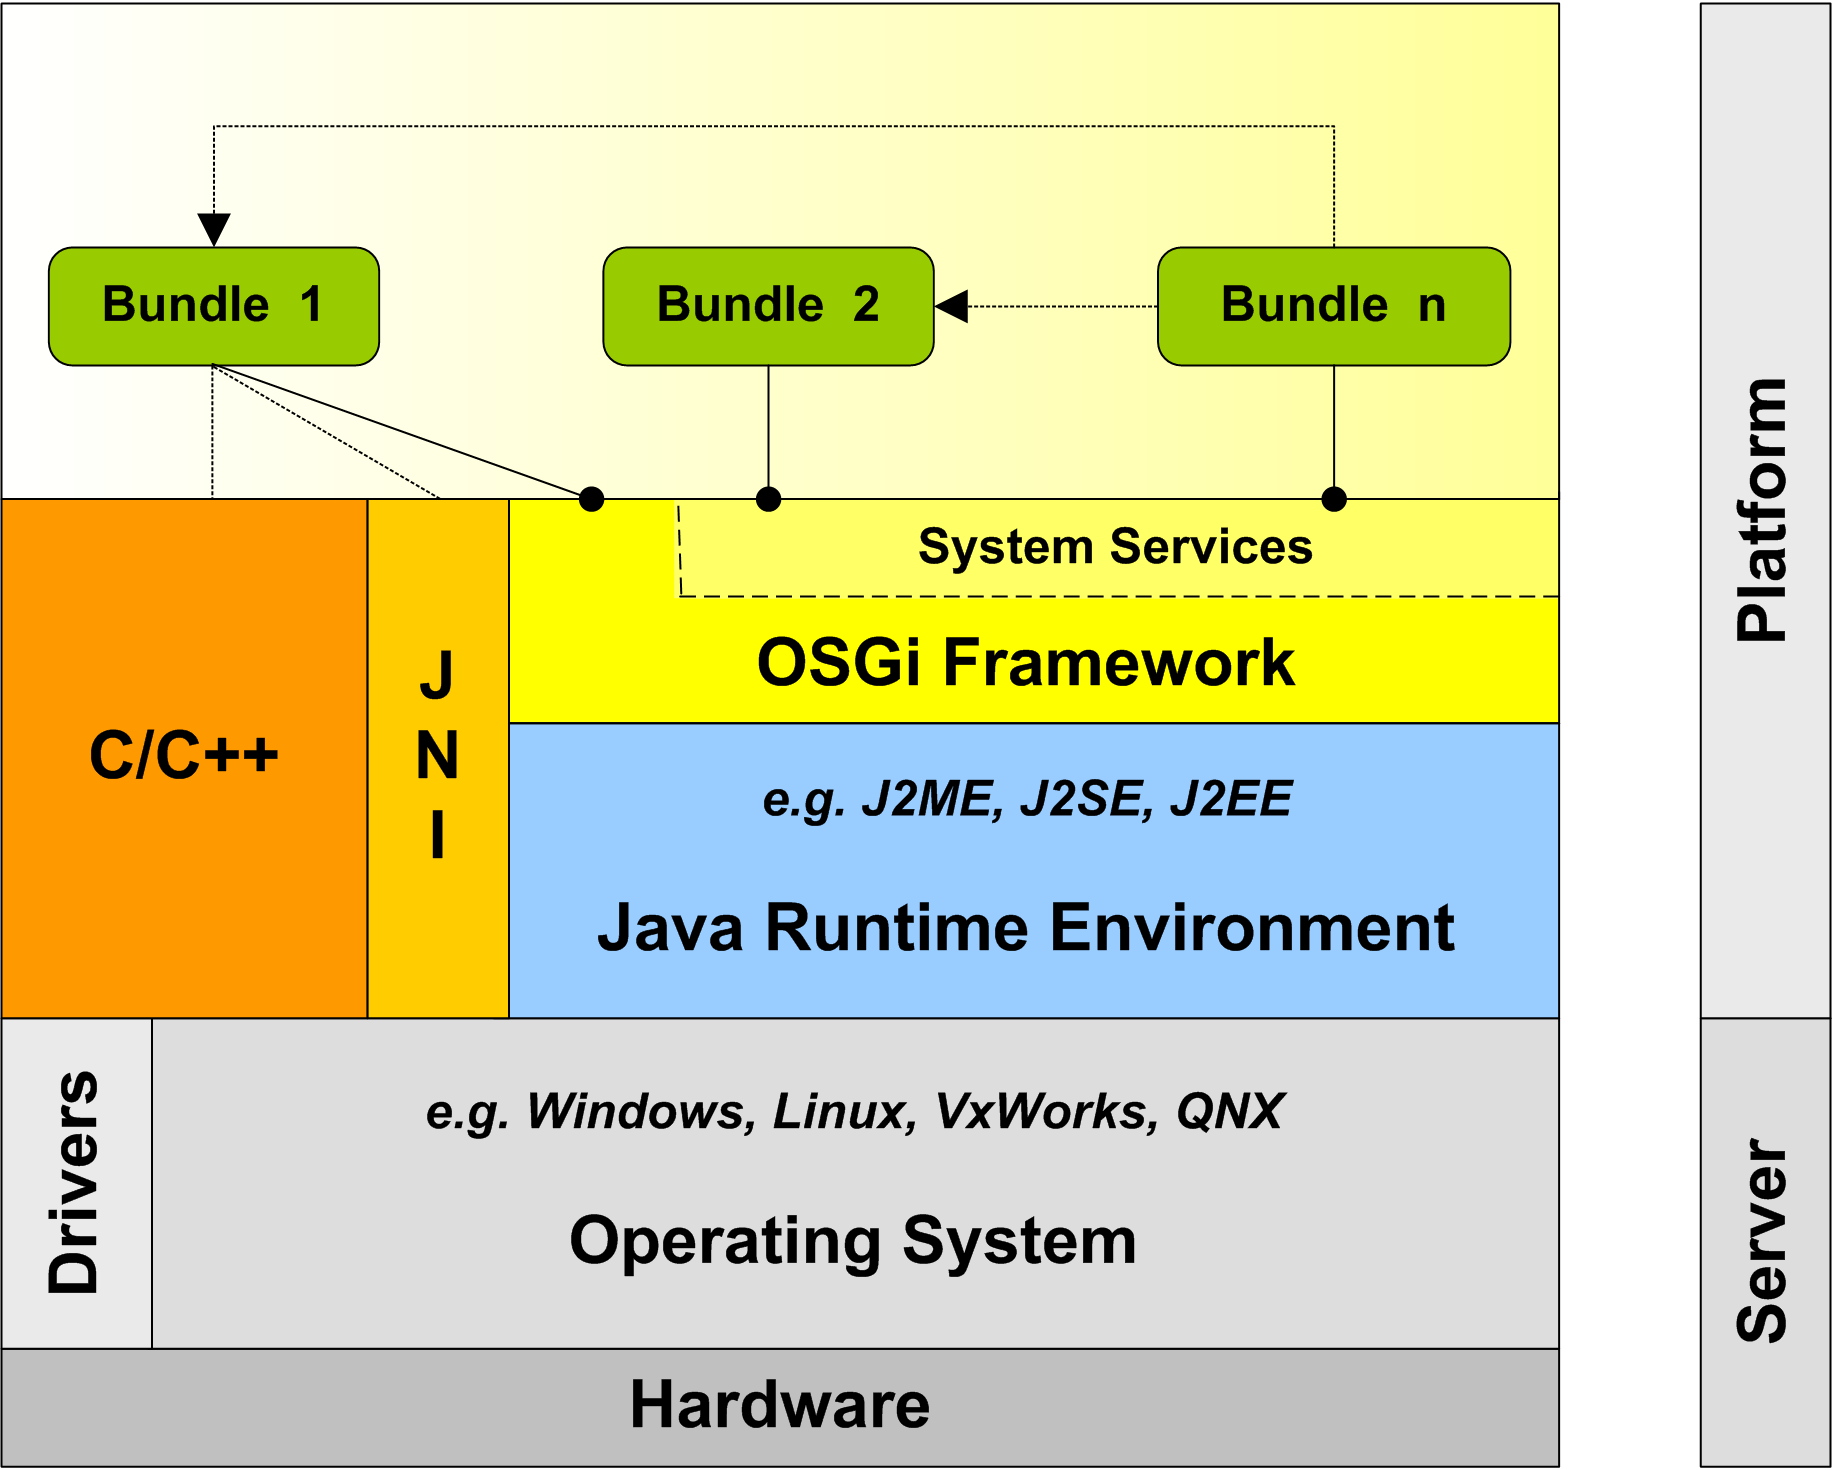
\includegraphics[scale=1.3]{pics/osgi_layer.png}
	\caption[OSGi Schichtenmodel]{
	\textbf{OSGi Schichtenmodel}
	}
	\end{center}
	\label{fig:osgi_layer}
\end{figure}

Die serviceorientierte Architektur der Pipeline wird also durch das
\name{OSGi Framework} diktiert und stellt somit die unterste Schicht der
Architekturabstraktion der Pipeline dar.



\section{bioinformatische Methoden}
Wie bereits in Kapitel \ref{chp:softwarearchitektur} erläutert, sollen die in
der Anwendung verwendeten Methoden zur Annotation dynamisch als \name{Step}
implementiert werden. Die Pipeline ist somit nicht auf bestimmte Methoden
beschränkt, vielmehr sind diese direkt durch die in der Pipeline verwendeten
Steps definiert \seef{fig:pipesFilter21}.

Aufgrund der konkreten Problemstellung durch die Zielsetzungen bezüglich der
Annotation von \name{C. higginsianum}, sowie als \name{Proof of Concept},
sollen einige, speziell auf die Annotation von \name{C. higginsianum} und den
hierzu verfügbaren Daten abgestimmte Steps implementiert werden.
\index{\name{C. higginsianum}|see\name{Colletotrichum higginsianum}}
Dabei soll die Annotation vorrangig \first{intrinsisch} \seec{chp:intrinsisch}
erfolgen, da homologiebasierte Ansätze in diesem Fall aus verschiedenen Gründen
wenig vielversprechend sind:
\index{intrinsisch}
\index{homologiebasiert}
\begin{itemize}
\item \todo{datenbanken haben nix}
\item \todo{ähm\ldots wars das schon?}
\end{itemize}
Für die intrinsische Genvorhersage sollen \first{Conditional Random
Fields} \seec{chp:crf}, oder \first{Hidden Markov Models} \seec{chp:hmm} zum
Einsatz kommen.
\index{Conditional Random Field}
\index{Hidden Markov Model}
Diese Verfahren, insbesondere \name{Conditional Random Fields}, stellen zum
jetztigen Zeitpunkt die beste Möglichkeit zur intrinischen Annotation dar.
\todo{mehr?}

Das eigentliche gene finding soll durch verschiedene, weitere Ansätze
unterstützt, bzw, verfeinert werden:

\todo{mask repetitive elemente}

\todo{EST mapping}
 
